\documentclass[12pt]{article}

\usepackage[13643]{easymcm}  % Team control number
\usepackage{longtable}
\usepackage{booktabs}
\usepackage{algorithm}
\usepackage{algpseudocode}

\newcommand{\toB}[1]{\color{blue}#1\color{black}}

\problem{A}  % Problem number

\title{}  % Title

\begin{document}

\begin{abstract}

	Some random text
	
\end{abstract}

\maketitle
\tableofcontents

\section{Introduction}

	\subsection{Background}
	
	Dandelion is a very common plant with scientific name \textit{Taraxacum officinale}, which is stemless, lactiferous and perennial\autocite{stewart2002biology}.  We can find them at roadsides, in wild fields or at inconspicuous places.  Just imagine that these little herbs with beautiful yellow flowers have been evolving on this planet for about 30 million years\autocite{dandelionhistory} - even longer than we human beings!
	
	But currently they are labeled as an invasive plant.  \textbf{Invasive species} is a relative concept.  It means an alien species whose introduction does or is likely to cause economic or environmental harm or harm to human health.\autocite{defInvasive}.  In some regions, dandelions do have some traits that make them invasive.  They can adapt different environments.  They have high growth rate and spread fast. They are likely to cuddle together and crowd out desirable plants, particularly in lawns.  Also, they have deep taproots that enable them to pull available water out of the soil.  It is also mentioned that dandelions could cause significant economic damage and infestation of other crops worldwide\autocite{stewart2002biology}.
	
	To disclose the reason that dandelion becomes invasive, researchers have done many studies on how the environment affects dandelion.  Laboratory and field studies have discussed the impact of climatic factors on its growth. Laboratory studies have been conducted on the relationship between germination rate and ambiances, such as light and temperature\autocite{letchamo1996light}.  Field studies have also been conducted on the same topic, providing credibility for the theoretical conclusions\autocite{yoneda1991effects}.  Studies have provided insights on the drought tolerance of dandelions\autocite{brock2005drought}. In the meanwhile, soil pollution and geographic factors are also being considered\autocite{verhoeven2013geographic}.
	
	Researchers have also paid great attention to dandelion dispersal, which is a major way for dandelion propagation.  Past papers have analyzed the structure of dandelion seeds and the effects of humidity on their structure, which affected the dispersal speed\autocite{greene1989model}. Scientists have modeled the aerodynamics of the seeds and demonstrated the effects of wind speed and directions.  It has also been proved that updrafts could not be neglected\autocite{tackenberg2003dandelion}.
	
	Beside this particular species, researchers have discussed invasive species more generally.  Ecologists have used species native to the invaded range as ``control species'' in attempting to determine the traits associated with invasive plant species\autocite{muth2006traits}.  A protocol has been developed for categorizing non-native plants according to their negative impacts on biodiversity in a large area such as a state, nation, or ecological region\autocite{randall2008invasive}.  Some online tools like \href{https://www.imapinvasives.org/decision-analysis-tool}{PIMDAT}\autocite{PIMDAT} have been provided to help people make strategic decisions about invasive species control projects.  Currently we also have Best Management Practices (BMPs) to prevent the introduction and spread of invasive species\autocite{BMP}.
	
	Public databases play an important role in the research of invasive species, especially for plants. By conferring to some database, we can find plant data to study biological attributes of the invasive species\autocite{USDA}.  Another database for tracking introduced species provides a baseline for effective modeling of species trends and interactions, geospatially and temporally\autocite{US-RIIS}.  US Government's Open Data provides a lot of data for current invasive plants\autocite{DATAGOV}.
	\newpage
	
	\subsection{Problem Restatement}

	In this paper, we will solve 2 problems.
	
	\textbf{For the first problem}, we will predict the spread of dandelions within a year (360 days).  Suppose that a dandelion in its dispersal period happens to be adjacent to an open one-hectare plot of land.  We need to create a mathematical model to describe how the dandelion will spread its seeds and how its offspring will scatter on the land.  And we will have to consider the effect of various climatic conditions, such as temperate, arid, and tropical climates, on dandelion growth.
	
	\textbf{For the second problem}, we will need to devise an ``impact factor'' for invasive species.  We will formulate a mathematical model to determine this factor and apply it to dandelions and some other invasive plants.  We also need to make sure the plants are invasive in the regions we choose.

\section{Dandelion Spread Model}

	\subsection{Assumptions and Justifications}
	
		\begin{enumerate}
			
			\item \textbf{The initial dandelion is at the midpoint of the left edge of a one-hectare square plot of land.  Seeds blown out of the area are neglected.}
			\vspace{-0.125in}
			\begin{description}
				\item[Justification:] According to the problem, the initial dandelion is adjacent to an open one-hectare plot of land. In order to acquire maximum spread effect, we set the plant in the middle of the left edge and make the right side our spread area. The seeds drifting to the left of the edge will be neglected. We may imagine a river or a forest is at the left side, so seeds cannot spread back to the area.
			\end{description}
			
			\item \textbf{The field is planar.}
			\vspace{-0.125in}
			\begin{description}
				\item[Justification:] We only consider the case of flat terrain.  This helps us limits the spread to two dimensions.  Flat terrain simplifies the calculation of dispersal distance since the wind can be at a constant height and the seed landing will not be affected by different topography.
			\end{description}
			
			\item \textbf{There are no other plants in the spread area.}
			\vspace{-0.125in}
			\begin{description}
				\item[Justification:] Considering other plants would add complicity to our model, for example, we need to collect data of those plants and study the competitive interactions between plants.  So simplification is necessary.
				
				More specifically, we assume that no other plants hinder the spread of dandelions, which means:
				
				\textbf{a.} Dandelion seeds are not intercepted by other plants;
				
				\textbf{b.} Dandelions do not have to compete with other plants.  
				
			\end{description}
			
			\item \textbf{Wind direction is uniformly distributed from 0$^\circ$ to 360$^\circ$.}
			\vspace{-0.125in}
			\begin{description}
				\item[Justification:] \label{assumption:wind} Wind speed and direction can be affected by different topography, especially near the land. At the height of dandelions, there could be vortices and updrafts that will greatly affect dispersal.  Though we can obtain wind data from meteorological stations, the data may not be accurate for a  small area. Therefore, we decided not to use the real-time wind direction data.
				
				Moreover, though wind rose maps provide the probabilities for each direction, without knowing the orientation of the edge, we cannot decide the relative wind direction to this area.  So we assume wind direction is uniformly distributed from 0$^\circ$ to 360$^\circ$. In this way, all directions have same odds and we can pin the dandelion on an arbitrary edge.
			\end{description}
			
			\item \textbf{Dandelion number always increases.}
			\vspace{-0.125in}
			\begin{description}
				\item[Justification:] More specifically, we assume that there are none of the followings.
				 
				 \textbf{a.} Human intervention;
				 
				 \textbf{b.} Natural enemies;
				 
				 \textbf{c.} Extreme weather conditions.
				
				This assumption simplifies our model.  Without considering above conditions, it will be an carefree place for dandelion growth.  And if we notice that the dandelion is a perennial herb, it is safe to assume the number will always increase .
			\end{description}
			
		\end{enumerate}
		
	
	

	
	\subsection{Model Overview}
		
		We will use a Monte Carlo simulation model to solve the problem.
		
		In reality, we find that sometimes dandelions grow in clusters, and at other times they are very sparse. Actually the spread process is affected by many random factors, including climate condition, wind speed and direction, topographical features and so on.  In order to eliminate this randomness, we need a method to find statistical patterns from repeating the process many times.  Candidates are neural network, deep learning, stochastic process, etc.  Among them, the Monte Carlo method becomes an option due to its simplicity.  Its underlying concept is to introduce randomness to solve problems.   It relies on repeated random sampling to obtain numerical results.  We will simulate dandelion spread process by going through the process many times, observing the results from a statistical perspective and drawing some conclusions.
		
		As the input for our model, we consider five environmental factors, as shown in \textbf{Table \ref{tb:vars}}.  
		
		{
			\fontsize{10}{14}\selectfont
			{
				\begin{longtable}{ccc}
					\caption{Environmental factors}
					\label{tb:vars}\\
					\toprule
					Symbol&Description&Unit\\
					\toprule
					$\mu_T$&Mean temperature&$^\circ$C\\
					$\sigma_T$&Standard deviation of temperature&$^\circ$C\\
					$\mu_W$&Mean wind speed&m/s\\
					$\sigma_W$&Standard deviation of wind speed&m/s\\
					$\mu_H$&Mean humidity&\%\\
					\bottomrule
				\end{longtable}
			}
		}
		
		And we will do the following to consider the environment influence to the dandelion spread process.
		
		\begin{itemize}
			\vspace{-0.5cm}
			\item Construct a temperature curve in \textbf{Section \ref{sec:temp}}.  
			
			\vspace{-0.2cm}
			\item Model dispersal mechanism in \textbf{Section \ref{sec:wind}}.
			
			\vspace{-0.2cm}
			\item Introduce an adaptation factor $k$ in \textbf{Section \ref{sec:af}}.  
		
		\end{itemize}
	
		\vspace{-0.5cm}
		Then our model will simulate the spread of dandelions by tracking every single dandelion according to a life cycle pattern, which we will model in \textbf{Section \ref{sec:life}}.  
		
		Next, we will choose 6 locations in the US.  For each location, we have one set of 5 input factors. We will run our model in 2 phases.  In the first phase, we will run 1000 times to get the optimal starting date for each location.  In the second phase, we will fix the starting date we get from the first phase and run another 1000 times to get the final ouput.
		
		We choose to run 1000 times because we find that the data with 1000 runs will exhibit an approximately normal distribution with a small margin of error for the mean.

		As the output of our model, we get all the dandelion locations for each day within 360 days.  
		
		In order to depict the statistical characteristics of dandelion spread, we conclude all the locations into 2 variables -- one is the \textbf{number} of dandelions and the other is the \textbf{mean distance} of dandelions from the initial one.  The first variable reflects spread intensity and the second one reflects spread range.


	
	\subsection{Temperature Curve}
	\label{sec:temp}
	
		\begin{wrapfigure}{r}{0.475\textwidth}
			\vspace{-0.4cm}
			\centering
			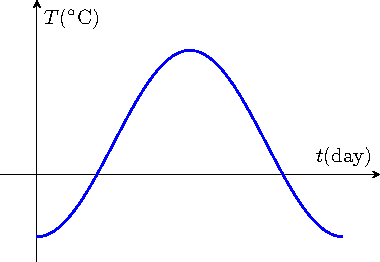
\includegraphics{fig-temperature_curve.pdf}
			\caption{Temperature curve}
			\label{fig:temp}
		\end{wrapfigure}
		
		We assume that the temperature follows a sinusoidal curve, as shown in \textbf{Fig.\ref{fig:temp}}.  We only consider locations in the northern hemisphere, so we further assume that the lowest temperature is reached on Jan.1st, when time $t = 0$.  We observe that the period of the curve is 360 (for convenience, we set each month to 30 days).  Thus, we write the equation as:
		
		\[
			T = -A \cos{\frac{2\pi}{360} t} + B.
		\]
		
		These conditions should be satisfied:
		
		\[
			\mu_T = \frac1{360} \int_0^{360} (-A \cos{\frac{2\pi}{360} t} + B) \, \mathrm{d}t,
		\]
		
		\[
			\sigma_T^2 = \frac1{360} \int_0^{360} \left[ (-A \cos{\frac{2\pi}{360} t} + B) - \mu_T \right] ^2 	\mathrm{d}t.
		\]
		
		Solving for $A$ and $B$, we get
		
		\begin{equation} \label{eq:temp}
			T = -\sqrt2 \sigma_T \cos{\frac{2\pi}{360} t} + \mu_T.
		\end{equation}





	\subsection{Dispersal Mechanisms}
	\label{sec:wind}
		
		For the \textbf{direction} of seed dispersal, we assume that the seed always follows the direction of the wind, which is uniformly distributed from 0$^\circ$ to 360$^\circ$ according to \textbf{Assumption \ref{assumption:wind}}.  
		
		For the \textbf{distance} of seed dispersal, we consider two types of wind, horizontal wind and updraft\autocite{tackenberg2003dandelion} (see \textbf{Fig.\ref{fig:dispersal}}).  The seed travels either a normal distance $s_N$ due to horizontal wind or a long distance $s_L$ due to updraft.  We set dispersal \textbf{distance} as the greater one between $s_N$ and  $s_L$.
		
		\begin{figure}[htbp]
			\centering
			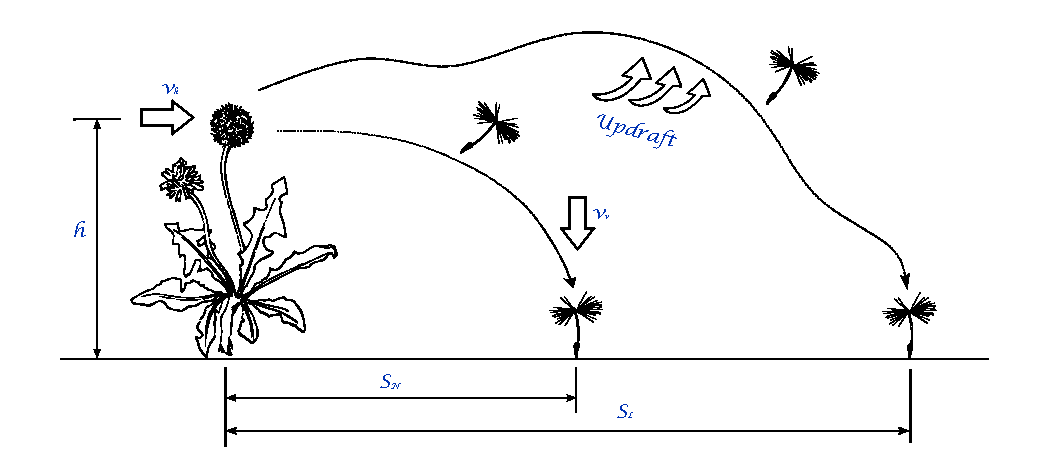
\includegraphics {wind_mode.pdf}
			\caption{Dandelion dispersal distance}
			\label{fig:dispersal}
		\end{figure}
		
		\subsubsection{Normal Distance $s_N$}
		
		In the case of horizontal wind, we have
		\begin{equation}\label{eq:hwind}
		 \frac{s_N}{v_h} = \frac{h}{v_v},
		\end{equation}
		where:
		
		$h$ is the height of the puffball, which is evaluated in \textbf{Section \ref{sec:life}};
		
		$v_v$ is the vertical component of the velocity of the seed, which is a constant value, 0.4 m/s\autocite{tackenberg2003dandelion}.
		
		$v_h$ is the speed of the horizontal wind, which follows a normal distribution with mean equals $\mu_W$ and standard deviation equals $\sigma_W$;

		\subsubsection{Long Distance $s_L$}
	
		\begin{wrapfigure}{r}{0.5\textwidth}
			\vspace{-1.5cm}
			\centering
			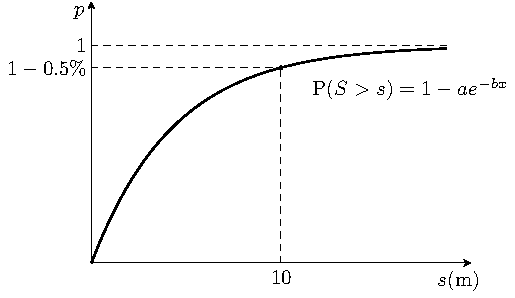
\includegraphics{fig-wind_curve.pdf}
			\caption{Cumulative distribution function of\\long-distance dispersal}
			\label{fig:longDistance}
		\end{wrapfigure}
		
		In the case of updraft, we suppose that $s_L$ follows an exponential distribution\autocite{okubo1989theoretical} with cumulative distribution function $\mathrm{P} (s_L < s) = 1 - ae^{-bs}$.  We know $\mathrm{P} (s_L < 0) = 0$.  We also know that the probability of a seed being blown further than 10 meters is 0.5\%\autocite{tackenberg2003dandelion}.  Therefore we can get:
		
		\begin{equation}\label{eq:updraft}
			\mathrm{P} (s_L < s) = 1 - e^{-0.53 s}.
		\end{equation}
		
		\newpage
		\subsubsection{Dandelion Density}
		
		The leafs of dandelions have a radius of around 15cm.  If a seed lands without falling on the leaf of another dandelion, the dandelion density should be less than $(1/0.15)^2$ = 45 plants/m$^2$.  If a seed arrives at a location whose vicinity has a density greater than this maximum value, the seed fails to land, which means it is not counted in our model.
		
		
		
		
		
	\subsection{Adaptation Factor}
	\label{sec:af}
		
			We introduce an adaptation factor $k$ which is evaluated by using $T$ and $\mu_H$.  Dandelions prefer temperate climates and relatively high humidity.  We divide temperature into three ranks, which indicate if the temperature is suitable for the dandelion.  We also divide humidity into three ranks, which indicate if the humidity is suitable for the dandelion.  On a given day, we calculate $k$ by computing the arithmetic mean of the rank for temperature and humidity and scaling $k$ so that $0 \leq k \leq 1$.
			
			We use $k$ to determine the mean value of some parameters of dandelions, such as the height of the puffball.  To allow for some variation, we let the parameters follow normal distributions with:
			\begin{equation}\label{eq:mu_p}
				\mu_{\mathrm{parameter}} = \left( \mathrm{worst} + \frac{\mathrm{best} - \mathrm{worst}}4 \right) + k \frac{\mathrm{best} - \mathrm{worst}}2, 
			\end{equation}	
			\begin{equation}\label{eq:sigma_p}
				\sigma_{\mathrm{parameter}} = \frac{\mathrm{best} - \mathrm{worst}}{12}.
			\end{equation}
			The worst and best values for the relevant parameters will be given in \textbf{Section \ref{sec:life}}.  If the a parameter exceeds the limits, it is set to the limit.
		
		
		
		
		
	\subsection{Dandelion Life Cycle}
	\label{sec:life}
		
		A dandelion can transfer between 6 states: \textbf{seed}, \textbf{developing}, \textbf{dispersal}, \textbf{inter-dispersal}, \textbf{hold}, and \textbf{dormancy}.
		
		\begin{figure}[htbp]
			\centering
			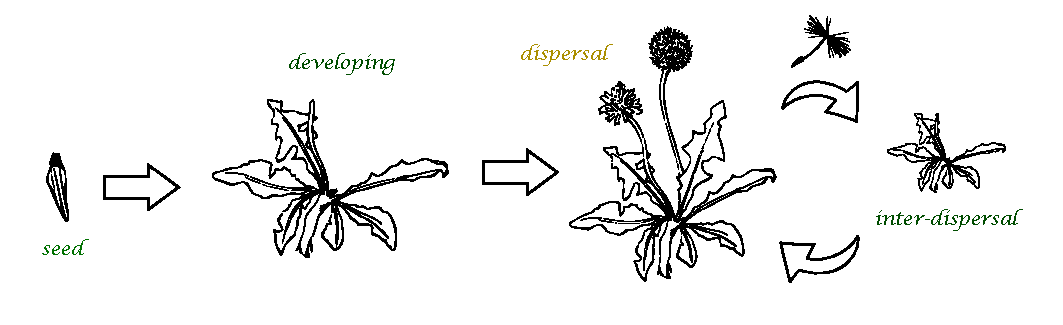
\includegraphics {life_cycle.pdf}
			\caption{Dandelion life cycle}
			\label{fig:lifeCycle}
		\end{figure}
		
		\begin{itemize}
			
			\item Out of all \textbf{seed}s, only 2\% will successfully germinate\autocite{honek2005post}.  These seeds will spend 3 days growing into the developing stage\autocite{stewart2002biology}.
			
			\item The \textbf{developing} stage is the time from sprouting to seed ripening.  It takes a sprout 60--95 days to grow into a flower, and an additional 9--12 days for the flower to ripen\autocite{gardenorganicNAripen}.  The exact duration of this stage is determined by the adaptation factor $k$ (worst = 107, best = 69) per \textbf{Section \ref{sec:af}}.
			
			\item The \textbf{dispersal} stage lasts 10 days.  A dandelion plant can produce around 10 seed heads per year and it usually flowers twice, so it produces 5 heads every time it flowers.  The number of seeds on each head is determined by $k$ (worst = 150, best = 200)\autocite{dukeNAdandelion}.  It takes each head 2 days to disperse its seeds.  The height of the puffball, $h$, is determined by $k$ (worst = 12, best = 40)\autocite{veggiegardenNAstem}.  The seeds are dispersed per the method stated in \textbf{Section \ref{sec:wind}}.
			
			\item The \textbf{inter-dispersal} stage is the stage between two dispersal stages of a plant.  In this stage, dandelions regrow their scapes and flowers.  Since most dandelions that flowered in spring usually flower again in fall\autocite{stewart2002biology}, the duration of this stage is set to be half a year, which is 180 days.   
			
		\end{itemize}
		We also consider two additional states, \textbf{hold} and \textbf{dormancy}.		
		\begin{itemize}
			
			\item When $T > 24^\circ$C, only 12.5\% of the flowers bloom and disperse their seeds\autocite{yoshie2020effects}.  We let dandelions enter dispersal by probability 12.5\% and move the rest into the \textbf{hold} stage.  In this stage, flowers are held in buds.  As soon as $T$ falls below $24^\circ$C, flowers can bloom and disperse seeds.  
		
			\item Dandelions enter the \textbf{dormancy} stage when $T < 0^\circ$C.  The temperature is low and it is likely that it snows.  All life activities of dandelions are paused.  As soon as $T$ rises above $0^\circ$C, dandelions resume the previous stage.
		
		\end{itemize}
		
		
		
		
		
	\subsection{Algorithm}
		\vspace{-0.4cm}
		{
			\fontsize{10}{14}\selectfont
			{
				\setlength{\parindent}{-1em}
				
				{
				\fontsize{12}{18}\selectfont
				\begin{longtable}{p{6.65in}}
					\toprule
					\textbf{Monte Carlo simulation algorithm for dandelion spread}\\
					\textbf{INPUT:} run times \toB{$n$ } and environment factors \toB{$\mu_T$}, \toB{$\sigma_T$}, \toB{$\mu_W$}, \toB{$\sigma_W$ } and \toB{$\mu_H$}\\
					\bottomrule
				\end{longtable}
				}
			
				\vspace{-0.5em}
				\begin{algorithmic}
					\For{1 to \toB{$n$}}
					\ForAll{\toB{$t$ } in days of one year}
					\State \toB{$T$ } $\gets$ evaluate current temperature per \textbf{Eq.\ref{eq:temp}}
					\State \toB{$k$ } $\gets$ evaluate adaptation factor per \textbf{Section \ref{sec:af}}
					\For{\toB{$dandelion$ } in current all dandelions}
					\State \textbf{if} \toB{$T$ } < 0 \textbf{then} \toB{$previous\,status$ } $\gets$ \toB{$current\,status$}, \toB{$current\,status$ } $\gets$ \textbf{Dormancy}
					\State \textbf{if} \toB{$current\,status$ } is \textbf{Dormancy} and \toB{$T$ } > 0 \textbf{then} \toB{$current\,status$ } $\gets$ \toB{$previous\,status$}
					\State \textbf{if} \toB{$current\,status$ } is \textbf{Hold} and \toB{$T$ } < 24 \textbf{then} \toB{$current\,status$ } $\gets$ \toB{$previous\,status$}
					
					\If{\toB{$current\,status$ } is \textbf{Developing} or \toB{$current\,status$ } is \textbf{Inter-dispersal}}
					\If{days of \toB{$current\,status$ } reaches the next stage}
					\If{\toB{$T$ } > 24}
					\State \toB{$current\,status$ } $\gets$ \textbf{Dispersal} with probability 0.125
					\If{\textbf{Dispersal} successfully}
					\State \toB{$current\,status$ } $\gets$ \textbf{Dispersal}
					\Else
					\State \toB{$previous\,status$ } $\gets$ \toB{$current\,status$}
					\State \toB{$current\,status$ } $\gets$ \textbf{Hold}
					\EndIf
					\Else
					\State \toB{$current\,status$ } $\gets$ \textbf{Dispersal}
					\EndIf
					\EndIf
					\EndIf
					
					\If{\toB{$current\,status$ } is \textbf{Seed}}
					\State \textbf{if} days of \toB{$current\,status$ } reaches the next stage \textbf{then} \toB{$current\,status$ } $\gets$ \textbf{Developing}
					\EndIf
					
					\If{\toB{$current\,status$ } is \textbf{Dispersal}}
					\State determine the seed count that needs to be dispersed
					\ForAll{\toB{$seed$ } in dispersing seeds}
					\State calculate dispersal distance per \textbf{Section \ref{sec:wind}}
					\State calculate land location and add it to \toB{$locations$ }
					\State generate a \toB{$new dandelion$ } with state \textbf{Seed}
					\EndFor
					\State \textbf{if} days of \toB{$current\,status$ } reaches the next stage \textbf{then} \toB{$current\,status$ } $\gets$ \textbf{Inter-dispersal}
					\EndIf
					
					
					\EndFor
					\EndFor
					\EndFor
					\State calculate \toB{$numbers$ } and \toB{$distances$ } per \toB{$locations$}
					\State \textbf{Return}{ \toB{$locations$ }, \toB{$numbers$ } and \toB{$distances$}}
				\end{algorithmic}
				
				{
				\fontsize{12}{18}\selectfont
				\begin{longtable}{p{6.6in}}
					\toprule
					\textbf{OUTPUT:} dandelion spread \toB{$locations$}, \toB{$numbers$ } and \toB{$mean\,distances$ } over days\\
					\bottomrule
				\end{longtable}
				}
			}
		}	
	
	\subsection{Dandelion Spread Results}
	
		\subsubsection{Location}
		
			We choose 6 locations in the US so that we have a variety of temperature and wind conditions.  AK is cold; CA, DC, and KS are warm; and FL and HI are relatively hot.  AK, DC, and KS have distinct seasons; CA and FL show moderate temperature fluctuations; and HI has very stable temperature.  The wind conditions also exhibit different patterns.  DC has notably large wind speed.  The values of the five environmental factors are listed in \textbf{Table \ref{tb:locs}}.  
			
			{
				\fontsize{10}{14}\selectfont
				{
					\begin{longtable}{ccccccc}
						\caption{Environmental factors for six locations}
						\label{tb:locs}\\
						\toprule
						State&Abbreviation&$\mu_T$ ($^\circ$C)&$\sigma_T$ ($^\circ$C)&$\mu_W$ (m/s)&$\sigma_W$ (m/s)&$\mu_H$ (\%)\\
						\toprule
						Alaska&AK&-0.05&9.08&7.27&1.42&81.46\\
						California&CA&16.20&4.99&6.02&0.90&80.36\\
						District of Columbia&DC&12.64&8.63&13.97&9.51&77.49\\
						Florida&FL&22.11&4.76&6.51&1.71&77.05\\
						Hawaii&HI&22.75&1.40&6.23&0.69&74.64\\
						Kansas&KS&12.58&9.98&8.58&1.55&79.37\\
						\bottomrule
					\end{longtable}
				}
			}
			\newpage
			
		\subsubsection{First Phase Results}	
			We run the model for 2 phases.
			
			In the first phase, we determine the optimal starting month of simulation.  For all 6 locations, we run the model with 12 cases that start respectively on the first day of each month, and get the number and mean distance for each case and each location.
			
			As an example, the results for Florida are shown in \textbf{Fig.\ref{fig:start}}.  The dandelion number varies greatly among the case, but the mean distance is approximately the same.  We can see that for Florida, we get the maximum dandelion number when the starting date is May 1st.  So we will use May as the starting month in the next phase.
			
			\begin{figure}[htbp]
				\centering
				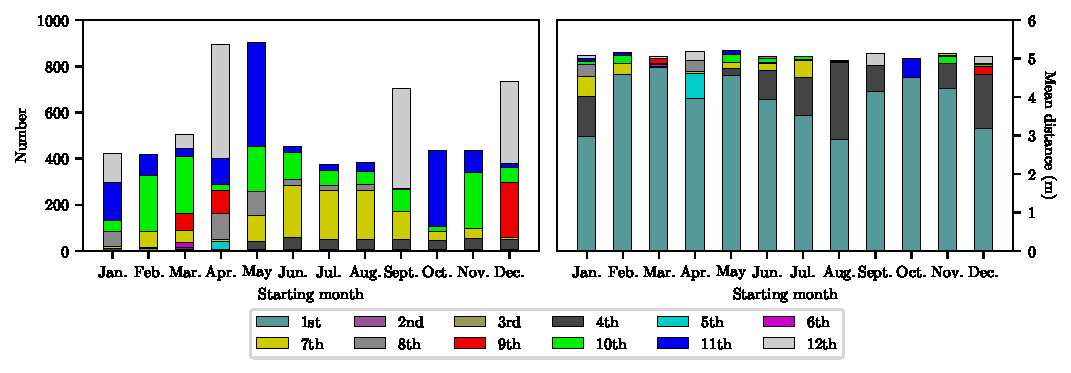
\includegraphics{start_month-number.pdf}
				\caption{Number and mean distance in Florida when simulation starts at different months}
				\label{fig:start}
			\end{figure}
			
			\textbf{Table \ref{tb:start}} lists all the data from the run of first phase.  The headers indicate the starting months, and the numbers in the table are the dandelion numbers at the end of 12 months.  The numbers corresponding to the optimal starting months are marked in blue.  In this way, we can determine that the optimal starting month is September for AK, August for CA, September for DC, May for FL, September for HI, and August for KS.
			
			{
				\fontsize{10}{14}\selectfont
				{
					\begin{longtable}{ccccccccccccc}
						\caption{Number at six locations when simulation starts at different dates}
						\label{tb:start}\\
						\toprule
						State&Jan.&Feb.&Mar.&Apr.&May&Jun.&Jul.&Aug.&Sept.&Oct.&Nov.&Dec.\\
						\toprule
						AK&74&79&70&35&44&75&43&49&\color{blue}\textbf{82}&72&74&75\\
						CA&547&567&545&532&585&561&544&\color{blue}\textbf{596}&564&566&581&563\\
						DC&1611&1589&1609&1563&1680&1657&1673&1733&\color{blue}\textbf{1808}&1696&1677&1658\\
						FL&424&417&505&895&\color{blue}\textbf{905}&453&375&384&706&436&435&736\\
						HI&519&329&610&593&586&596&308&543&\color{blue}\textbf{618}&383&385&600\\
						KS&823&276&268&405&548&274&266&\color{blue}\textbf{1067}&287&288&950&834\\
						\bottomrule
					\end{longtable}
				}
			}
			
			
			
		\subsubsection{Second Phase Results}
		
			In the second phase, we run the model 1000 times for each location beginning at the optimal starting month from the first phase.  The resulting frequency histogram for Florida is shown in \textbf{Fig.\ref{fig:freqDand}}.  We can see that both the number and the mean distance follow an approximately normal distribution.  
			
			\begin{figure}[htbp]
				\centering
				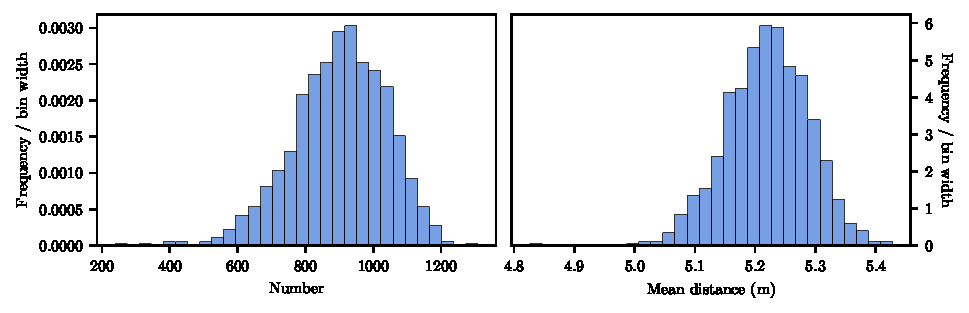
\includegraphics{number-frequency.pdf}
				\caption{Frequency distribution of number and mean distance in Florida}
				\label{fig:freqDand}
			\end{figure}
			
			We calculated several statistical characteristics for each location, as shown in \textbf{Table \ref{tb:numDistribution}} and \textbf{Table \ref{tb:distDistribution}}.	 We examine the statistics for dandelion number.  The confidence interval of the mean is relatively small for all locations, which implies the mean is quite accurate.  The standard deviation and range are large, which shows that the spread of dandelions is easily affected by random factors such as fluctuations in the environment.  For all locations except California, the distributions are platykurtic.  For all locations except Alaska, the distribution is skewed to the left.  Its mass is concentrated on the right, so the dandelion number is slightly more likely to be greater than the mean rather than smaller.  However, because of the unfavorable environmental conditions in Alaska, the number is more likely to be smaller than the mean.
			
			{
				\fontsize{10}{14}\selectfont
				{
					\begin{longtable}{cccccccc}
						\caption{Descriptive statistics of number at six locations}
						\label{tb:numDistribution}\\
						\toprule
						Location&Mean&Standard Deviation&Kurtosis&Skewness&Range&Median&Confidence Level (95.0\%)\\
						\toprule
						AK&72.7&26.5&-0.11&0.38&150&71&1.64\\
						CA&595.1&82.48&3.78&-1.32&744&609&5.11\\
						DC&1780&484.9&-0.04&-0.03&3274&1772.5&30.1\\
						FL&886.4&140.4&1.04&-0.72&981&905&8.71\\
						HI&607.5&81.9&1.12&-0.79&565&617&5.08\\
						KS&1066&186.4&1.05&-0.72&1403&1096&11.6\\
						\bottomrule
					\end{longtable}
					
				}
			}
			
			{
				\fontsize{10}{14}\selectfont
				{
					\begin{longtable}{cccccccc}
						\caption{Descriptive Statistics of the mean distance at six locations}
						\label{tb:distDistribution}\\
						\toprule
						Location&Mean&Standard Deviation&Kurtosis&Skewness&Range&Median&Confidence Level (95.0\%)\\
						\toprule
						AK&4.29&0.18&0.44&0.25&1.28&4.29&0.01\\
						CA&4.52&0.09&0.51&-0.53&0.67&4.52&0.01\\
						DC&11.84&0.21&1.5&-0.51&1.93&11.85&0.01\\
						FL&5.21&0.07&1.91&-0.64&0.66&5.21&0.00\\
						HI&4.99&0.08&0.138&-0.27&0.5&4.99&0.00\\
						KS&6.52&0.05&0.8&-0.36&0.44&6.52&0.00\\
						\bottomrule
					\end{longtable}
				}
			}
			
			Out of the 1000 runs, we select the run that has a dandelion number closest to the mean value.  The positions and current stages of the dandelions at the end of 12 months are shown in \textbf{Fig.\ref{fig:scatter5loc}}.  For all locations except the District of Columbia, most dandelions grow in a semicircular ring centered at the origin.  Alaska is apparently unsuitable for dandelions to spread.  In California, Hawaii, Florida, and Kansas, dandelions all spread to a moderate range.
			
			\begin{figure}[htbp]
				\centering
				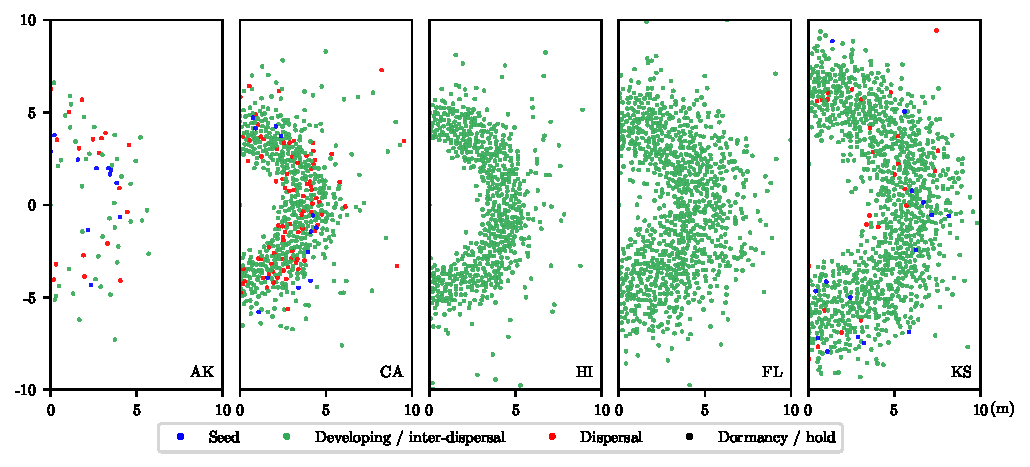
\includegraphics{spread_course-location_non_DC.pdf}
				\caption{The spread at the end of 12 months at different locations}
				\label{fig:scatter5loc}
				
				\vspace{1cm}

				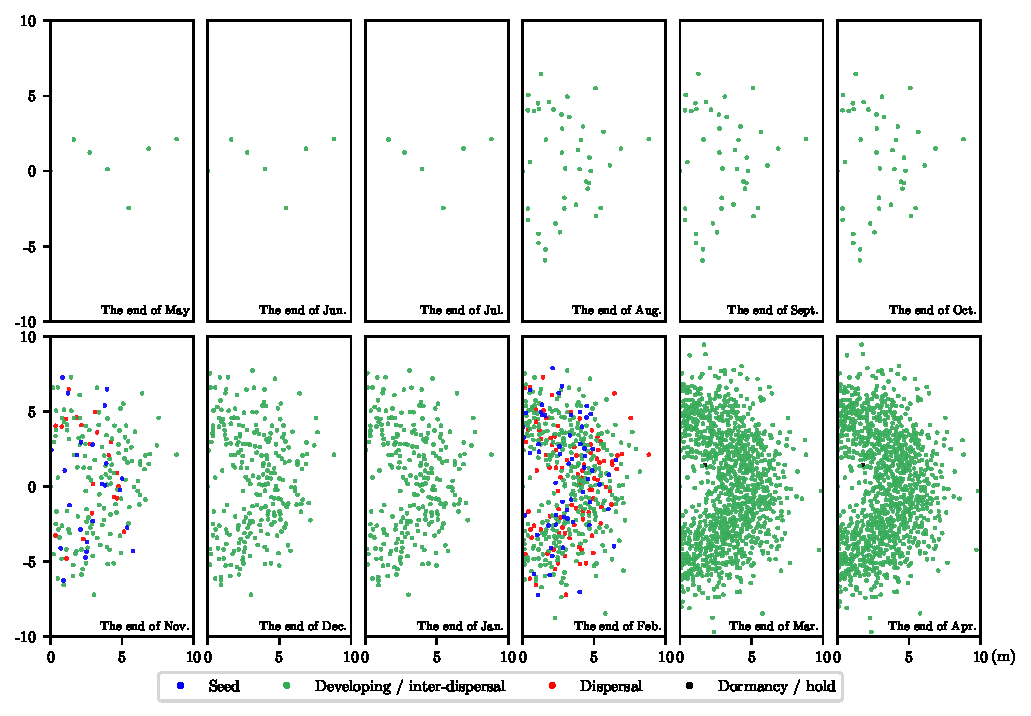
\includegraphics{spread_course-time.pdf}
				\caption{The spread during 12 months in the District of Columbia}
				\label{fig:spreadDC}
			\end{figure}
			\newpage
			
			District of Columbia has the most dandelions at the of 12 months.  We plotted dandelion spread at the end of each month this location (see \textbf{Fig.\ref{fig:spreadDC}}) so that it can be clearly seen how the dandelions spread in the course of time.  Compared to other locations, District of Columnbia has greater wind speed so the dandelions spread much further and they form a semicircle instead of a ring.  The closer to the origin, the denser the plants.  Additionally, there is a sudden increase every three months, which is caused by the flowering of a new generation of dandelions.
			
			Finally, we draw a graph of the natural logarithm of dandelion number in \textbf{Fig.\ref{fig:time}}.  The lines have several jumps and platforms.  The dandelion number increases exponentially at the end of each fixed period.  This conclusion coincides with our observation in \textbf{Fig.\ref{fig:spreadDC}}.  Again, Alaska is different.  Dandelions there are dormant in the first three months of the year, and eventually produce fewer offspring than other locations.
			
			\begin{figure}[htbp]
				\centering
				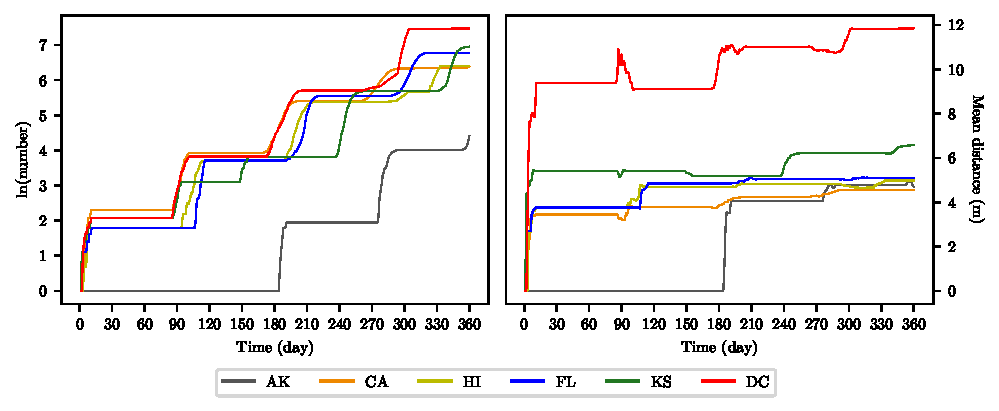
\includegraphics{number_mean_distance-time.pdf}
				\caption{Number and mean distance over time}
				\label{fig:time}
			\end{figure}
		
		
		
		\subsubsection{Sensitivity Analysis}
			
			We conduct a sensitivity analysis on the five factors from \textbf{Table \ref{tb:vars}} by varying one of them while keeping the other four fixed.  
			
			\textbf{Fig.\ref{fig:saT}} shows the results for temperature.  When $\mu_T$ falls below 7$^\circ$C or rises above 23$^\circ$C, dandelion number decreases sharply.  This is because dandelions are transferred to the dormancy or hold stages at certain temperatures.  The number is very sensitive to extreme temperatures, but only moderately sensitive to mild temperatures.  The mean distance increases with $\mu_T$ up to 19$^\circ$C, where the it temporarily levels off and begins to fall at 23$^\circ$C.  It has medium sensitivity to $\mu_T$.
			
			Both number and mean distance decreases as $\sigma_T$ increases.  They decrease relatively slowly below $\sigma_T = 5^\circ$C and rapidly above that value.  However, the overall sensitivity is not high for either number or mean distance.
			
			\begin{figure}[htbp]
				\centering
				\begin{minipage}{0.04\textwidth}\end{minipage}
				\begin{minipage}{0.46\textwidth}
					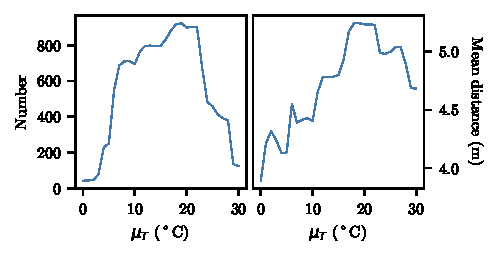
\includegraphics{sa_MuT.pdf}
				\end{minipage}
				\begin{minipage}{0.46\textwidth}
					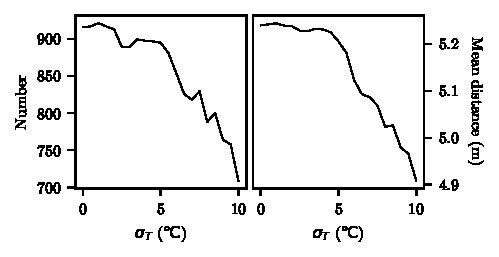
\includegraphics{sa_StdT.pdf}
				\end{minipage}
				\begin{minipage}{0.04\textwidth}\end{minipage}
				\caption{Sensitivity analysis: temperature}
				\label{fig:saT}
			\end{figure}
			
			\textbf{Fig.\ref{fig:saW}} shows the results for wind speed.  The number and mean distance have a positive correlation with $\mu_W$ and $\sigma_W$ and change drastically when the two factors vary.  When $\mu_W$ increases, seeds are dispersed farther and land further apart from each other.  When $\sigma_W$ increases, there is greater variation in dispersal distance.  In both cases it is less likely for seeds to land on other plants, making dandelion number rise quickly.
			
			\begin{figure}[htbp]
				\centering
				\begin{minipage}{0.04\textwidth}\end{minipage}
				\begin{minipage}{0.46\textwidth}
					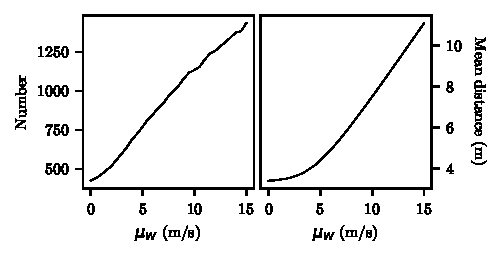
\includegraphics{sa_MuW.pdf}
				\end{minipage}
				\begin{minipage}{0.46\textwidth}
					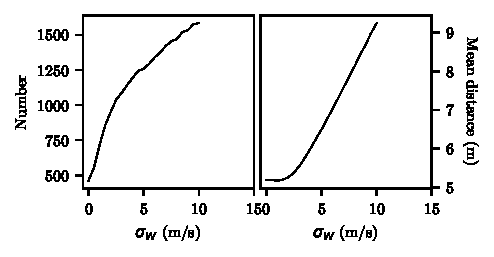
\includegraphics{sa_StdW.pdf}
				\end{minipage}
				\caption{Sensitivity analysis: wind speed}
				\label{fig:saW}
			\end{figure}
			
			\textbf{Fig.\ref{fig:saH}} shows the results for humidity.  There are three levels of number and mean distance corresponding to different humidity.  This is because of the three ranks for humidity that are used in the calculation of the adaptation factor $k$, see \textbf{Section \ref{sec:af}}.
			
			\begin{figure}[htbp]
				\centering
				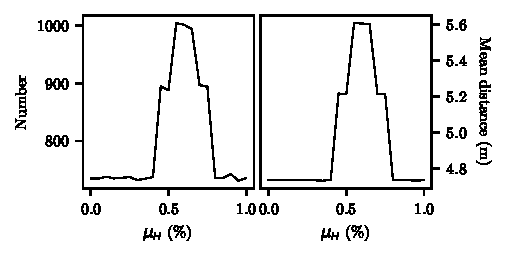
\includegraphics{sa_Hum.pdf}
				\caption{Sensitivity analysis: humidity}
				\label{fig:saH}
			\end{figure}
			
			
			
		\subsubsection{Strengths and Weaknesses}
		
			\paragraph{Strengths}
			\vspace{-0.1cm}
			\begin{itemize}
				\vspace{-0.3cm}
				\item Our model is \textbf{realistic}.  We used data for real locations.  And we considered how environmental factors and random variations contribute to dandelion spread.  Besides, we tracked every plant during the entire spread process.  
				
				\vspace{-0.3cm}
				\item Our model is \textbf{easy to understand and implement}.  The simulation method is very intuitive, and the model only requires five input values that are easily acquired from meteorological databases.
				
				\vspace{-0.3cm}
				\item Our model is \textbf{extensible}.  We can easily consider other factors by adding a component to the model.  For example, if we want to consider the effect of rain, we can determine the effects of rain on the different stages of dandelions and add this new component to our current model.
			\end{itemize}
			
			\paragraph{Weaknesses}
			\vspace{-0.5cm}
			\begin{itemize}
				\vspace{-0.3cm}
				\item Our model is \textbf{time-intensive}.  To get a fairly accurate result, we have to run about 1000 times for each location.  Compared to other possible models, the efficiency of our model is relatively low.
				
				\vspace{-0.3cm}
				\item The \textbf{adaptation factor} may be an over-simplification.  It may not represent the reality very accurately.  If we can acquire the relationship between dandelion parameters and climate conditions, we will be able to substitute the adaptation factor with some more accurate components.
				
				\vspace{-0.3cm}
				\item Our model \textbf{misses certain factors}.  We did not consider rain, which stops flowers from blooming and hinders seed dispersal.  Other missed factors include interactions with other plants and human intervention.  These can be added as new components in the future.
				
			\end{itemize}

		
		
		
		
\section{Plant Impact Factor Model}

	\subsection{Assumptions and Justifications}
	
	\subsection{Model Description}

		hello
		
		{
			\fontsize{10}{14}\selectfont
			{
			\begin{longtable}{p{0.2in}p{1.5in}p{4.3in}}
				
				\caption{Attributes}
				\label{tb:attributes}\\
				
				\toprule
				\multicolumn{1}{c}{\textbf{Symbol}} 
					& \multicolumn{1}{c}{\textbf{Attributes}}
					& \multicolumn{1}{c}{\textbf{$a_i$, $b_i$ and $c_i$ Evaluation}} \\
			
				\toprule
				\multicolumn{3}{l}{Category $A$ - Plant Characteristics}\\
				\midrule
				
				$A_1$ & Duration & $a_1=0.5$ (Annual), $0.75$ (Biennial), $1$ (Perennial)\\
				$A_2$ & Growing Habit & $a_2=0$ (Tree), $0.25$ (Shrub), $0.5$ (Vine), $0.75$ (Graminoid), $1$ (Forb/herb)\\ 
				$A_3$ & Growth Rate & The growth rate after successful establishment\\
					&& $a_3=0.5$ (Slow), $0.75$ (Moderate), $1$ (Rapid)\\
				$A_4$ & Lifespan & $a_4=0.25$ (when $a_1=0.5$ or $0.75$), $0.5$ (Short), $0.75$ (Moderate), $1$ (Long) \\
				$A_5$ & Fertility Requirement & Relative level of nutrition (N, P, K) required for normal growth and development.\\
					 && $a_5=0.5$ (Low), $0.75$ (Medium), $1$ (High)\\
				$A_6$ & Fruit/Seed Abundance & The amount of seed produced.\\
					&& $a_6=0.25$ (None), $0.5$ (Low), $0.75$ (Medium), $1$ (High)\\
				$A_7$ & Propagated Methods & The propagetion methods number, $n_7$. The methods can be Propagated by Bare Root, by Bulb, by Container, by Corm, by Cuttings, by Seed, by Sod, by Sprigs, or by Tubers. \\
					&& $a_7=0.25$ ($n_7=1$), $0.5$ ($n_7=2$), $0.75$ ($n_7=3$), $1$ ($n_7\geq4$)\\
				$A_8$ & Seed Spread Rate & The capability of the plant to spread through its seed production.\\
					&& $a_8=0.25$ (None), $0.5$ (Slow), $0.75$ (Moderate), $1$ (Rapid)\\
				$A_9$ & Seedling Vigor & The expected seedling survival percentage of the plant\\
					&& $a_9=0.5$ (Low), $0.75$ (Medium), $1$ (High)\\
				
				\midrule
				\multicolumn{3}{l}{Category $B$ - Human and Environment}  \\
				\midrule
				
				$B_1$ & Toxicity & The relative toxicity of the plant to either humans or livestock.\\
					&& $b_1=0$ (None), $0.5$ (Slight), $0.75$ (Moderate), $1$ (Severe)\\
				$B_2$ & Product & The level of the plant known to be suitable for multiple types of products.\\
					&& $b_2=0$ (Copiousness), $0.25$ (Many), $0.5$ (Some), $0.75$ (few), $1$ (None)\\
				$B_3$ & Palatable Animal & The relative palatability of this plant to browsing animals or to grazing animals.\\
					&& $b_3=0$ (High), $0.5$ (Moderate), $0.75$ (Low), $1$ (None)\\
				$B_4$ & Palatable Human & The plant produce berries, nuts, seeds, or fruits are palatable to humans. \\
					&& $b_4=0.5$ (Yes), $1$ (No)\\
				$B_5$ & Commercial Availability & The plant propagules are in the commercial marketplace \\
					&& $b_5=0.5$ (Yes), $1$ (No)\\
			
				\midrule
				\multicolumn{3}{l}{Category $C$ - Location}  \\
				\midrule
				
				$C_1$ & Soil Adaptation & The soil adaptation level\\
				&& $c_1=0$ (Low), $0.5$ (Medium), $1$ (High)\\
				$C_2$ & Temperature Adaptation & The temperature adaptation level\\
				&& $c_2=0$ (Low), $0.5$ (Medium), $1$ (High)\\
				$C_3$ & Humid Adaptation & The humid adaptation level\\
				&& $c_3=0$ (Low), $0.5$ (Medium), $1$ (High)\\
				$C_4$ & Population Density & The level of population density.\\
				&& $c_4=0$ (High), $0.5$ (Medium), $1$ (Low)\\
			
				\bottomrule
			
			\end{longtable}
			}
		}
		
		{
			\fontsize{10}{18}\selectfont
			{
				\begin{longtable}{c|ccccccccc|ccccc||cccc}
					
					\caption{AHP comparison matrix}
					\label{tb:mat}\\
					
					\toprule
					&$A_1$&$A_2$&$A_3$&$A_4$&$A_5$&$A_6$&$A_7$&$A_8$&$A_9$&$B_1$&$B_2$&$B_3$&$B_4$&$B_5$&$C_1$&$C_2$&$C_3$&$C_4$\\
					\toprule
					$A_1$&$1$&$1/3$&$1/7$&$1/3$&$1$&$1/7$&$1/4$&$1/7$&$1/5$&$1/9$&$1/5$&$1/3$&$1/4$&$1/4$&$1/5$&$1/5$&$1/5$&$1/3$\\
					$A_2$&$3$&$1$&$1/5$&$1$&$3$&$1/5$&$1/2$&$1/5$&$1/3$&$1/7$&$1/3$&$1$&$1/2$&$1/2$&$1/3$&$1/3$&$1/3$&$1$\\
					$A_3$&$7$&$5$&$1$&$5$&$7$&$1$&$4$&$1$&$3$&$1/3$&$3$&$5$&$4$&$4$&$3$&$3$&$3$&$5$\\
					$A_4$&$3$&$1$&$1/5$&$1$&$3$&$1/5$&$1/2$&$1/5$&$1/3$&$1/7$&$1/3$&$1$&$1/2$&$1/2$&$1/3$&$1/3$&$1/3$&$1$\\
					$A_5$&$1$&$1/3$&$1/7$&$1/3$&$1$&$1/7$&$1/4$&$1/7$&$1/5$&$1/9$&$1/5$&$1/3$&$1/4$&$1/4$&$1/5$&$1/5$&$1/5$&$1/3$\\
					$A_6$&$7$&$5$&$1$&$5$&$7$&$1$&$4$&$1$&$3$&$1/3$&$3$&$5$&$4$&$4$&$3$&$3$&$3$&$5$\\
					$A_7$&$4$&$2$&$1/4$&$2$&$4$&$1/4$&$1$&$1/4$&$1/2$&$1/4$&$1/2$&$2$&$1$&$1$&$1/2$&$1/2$&$1/2$&$2$\\
					$A_8$&$7$&$5$&$1$&$5$&$7$&$1$&$4$&$1$&$3$&$1/3$&$3$&$5$&$4$&$4$&$3$&$3$&$3$&$5$\\
					$A_9$&$5$&$3$&$1/3$&$3$&$5$&$1/3$&$2$&$1/3$&$1$&$1/5$&$1$&$3$&$2$&$2$&$1$&$1$&$1$&$3$\\
					\midrule
					$B_1$&$9$&$7$&$3$&$7$&$7$&$3$&$4$&$3$&$5$&$1$&$5$&$7$&$4$&$4$&$5$&$5$&$5$&$7$\\
					$B_2$&$5$&$3$&$1/3$&$3$&$5$&$1/3$&$2$&$1/3$&$1$&$1/5$&$1$&$3$&$2$&$2$&$1$&$1$&$1$&$3$\\
					$B_3$&$3$&$1$&$1/5$&$1$&$3$&$1/5$&$1/2$&$1/5$&$1/3$&$1/7$&$1/3$&$1$&$1/2$&$1/2$&$1/3$&$1/3$&$1/3$&$1$\\
					$B_4$&$4$&$2$&$1/4$&$2$&$4$&$1/4$&$1$&$1/4$&$1/2$&$1/4$&$1/2$&$2$&$1$&$1$&$1/2$&$1/2$&$1/2$&$2$\\
					$B_5$&$4$&$2$&$1/4$&$2$&$4$&$1/4$&$1$&$1/4$&$1/2$&$1/4$&$1/2$&$2$&$1$&$1$&$1/2$&$1/2$&$1/2$&$2$\\
					\midrule
					\midrule
					$C_1$&$5$&$3$&$1/3$&$3$&$5$&$1/3$&$2$&$1/3$&$1$&$1/5$&$1$&$3$&$2$&$2$&$1$&$1$&$1$&$3$\\
					$C_2$&$5$&$3$&$1/3$&$3$&$5$&$1/3$&$2$&$1/3$&$1$&$1/5$&$1$&$3$&$2$&$2$&$1$&$1$&$1$&$3$\\
					$C_3$&$5$&$3$&$1/3$&$3$&$5$&$1/3$&$2$&$1/3$&$1$&$1/5$&$1$&$3$&$2$&$2$&$1$&$1$&$1$&$3$\\
					$C_4$&$3$&$1$&$1/5$&$1$&$3$&$1/5$&$1/2$&$1/5$&$1/3$&$1/7$&$1/3$&$1$&$1/2$&$1/2$&$1/3$&$1/3$&$1/3$&$1$\\
					\bottomrule
				\end{longtable}
			}
		}	

		hello!!! \\

		{
			\fontsize{10}{14}\selectfont
			{
				\begin{longtable}{cccccccc}
					\caption{Consistency test}
					\label{tb:consistency}\\
					
					\toprule
					Impact Factor&Attribute Number&max eigenvalue 
					&\multirow{2}{*}{$\mathrm{CI}=\frac{\lambda_{max}-n}{n-1}$}
					&\multirow{2}{*}{$\mathrm{RI}$}
					&\multirow{2}{*}{$\mathrm{CR}=\frac{\mathrm{CI}}{\mathrm{RI}}$}
					&\multirow{2}{*}{$\mathrm{CR}<0.1?$}\\
					Type&$n$&$\lambda_{max}$\\
					\toprule
					Global&$14$&$14.501$&$0.0386$&$1.49$&0.0259&Yes\\
					Local&$18$&$18.561$&$0.0330$&$1.49$&0.0221&Yes\\
					\bottomrule
				\end{longtable}
			}
		}	

	hello!!! \\
	hello!!! \\
	hello!!! \\
	hello!!! \\
	
		{
			\fontsize{10}{14}\selectfont
			{
				\begin{longtable}{c|ccccccccc}
					\caption{Weights results}
					\label{tb:weights}\\
					
					\toprule
					Type&$\alpha_1$&$\alpha_2$&$\alpha_3$&$\alpha_4$&$\alpha_5$&$\alpha_6$&$\alpha_7$&$\alpha_8$&$\alpha_9$\\
					\toprule
					Global&0.014&0.027&0.134&0.027&0.014&0.134&0.044&0.134&0.066\\
					Local&0.011&0.021&0.113&0.021&0.011&0.113&0.034&0.113&0.052\\
					\toprule
					\toprule
					&$\beta_1$&$\beta_2$&$\beta_3$&$\beta_4$&$\beta_5$&$\gamma_1$&$\gamma_2$&$\gamma_3$&$\gamma_4$\\
					\toprule
					Global&0.227&0.066&0.027&0.044&0.044&-&-&-&-\\
					Local&0.192&0.052&0.021&0.034&0.034&0.052&0.052&0.052&0.021\\
					\bottomrule
				\end{longtable}
			}
		}	
	
		hello!!! \\
		
		{
			\fontsize{10}{14}\selectfont
			{
				\begin{longtable}{cccccc}
					\caption{Plant Rankings}
					\label{tb:ranks}\\
					
					\toprule
					Rank&Scientific Name&Vernacular Name&Duration&Growing Habit&IF$_g$\\
					\toprule
					1&Melilotus officinalis&Sweetclover&Perennial&Forb/herb&84.5\\
					2&Senecio vulgaris&Old-man-in-the-spring&Biennial&Forb/herb&83.3\\
					3&Ailanthus altissima&Tree of heaven&Perennial&Tree&81.8\\
					4&Crotalaria spectabilis&Showy rattlebox&Annual&Forb/herb&81.7\\
					5&Ranunculus repens&Creeping buttercup&Perennial&Forb/herb&80.8\\
					6&Melilotus indicus&Annual yellow sweetclover&Annual&Forb/herb&80.0\\
					7&Digitalis purpurea&Purple foxglove&Biennial&Forb/herb&79.9\\
					8&Sorghum halepense&Johnsongrass&Perennial&Graminoid&78.9\\
					9&Schedonorus arundinaceus&Tall fescue&Perennial&Graminoid&76.8\\
					10&Vicia sativa&Garden vetch&Annual&Forb/herb&73.8\\
					$\vdots$\\
					26&Taraxacum officinale&Common dandelion&Perennial&Forb/herb&66.9\\
					\bottomrule
				\end{longtable}
			}
		}
		
		remember to write the sample quantity and unit \\

		{
			\fontsize{10}{14}\selectfont
			{
				\begin{longtable}{ccccccc}
					\caption{Distribution of impact factor}
					\label{tb:IFDistribution}\\
					
					\toprule
					Mean&Standard Deviation&Kurtosis&Skewness&Range&Median&Confidence Level (95.0\%)\\
					\toprule
					57.9&8.65&0.81&0.41&50.51&57.25&1.13\\
					\bottomrule
				\end{longtable}
			}
		}
		
		hello!!! \\
		
		hello!!! \\

	\subsection{Sensitivity Analysis}
	
		\begin{figure}[htbp]
			\centering
			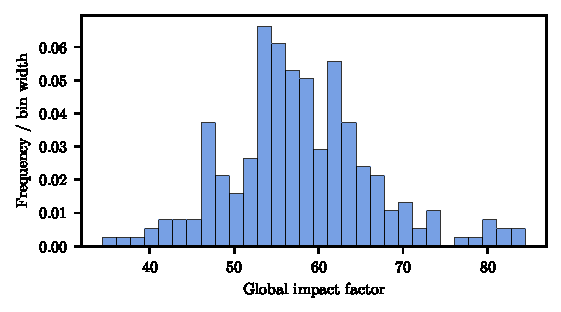
\includegraphics{IF-frequency.pdf}
			\caption{Frequency distribution of global impact factor}
			\label{fig:freqIF}
		\end{figure}
	
		\begin{figure}[htbp]
			\centering
			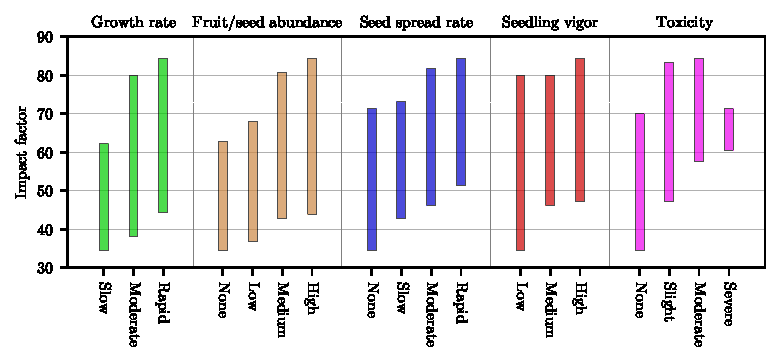
\includegraphics{categories-IF.pdf}
			\caption{Sensitivity analysis}
			\label{fig:IFfactors}
		\end{figure}
		
		\begin{figure}[htbp]
			\centering
			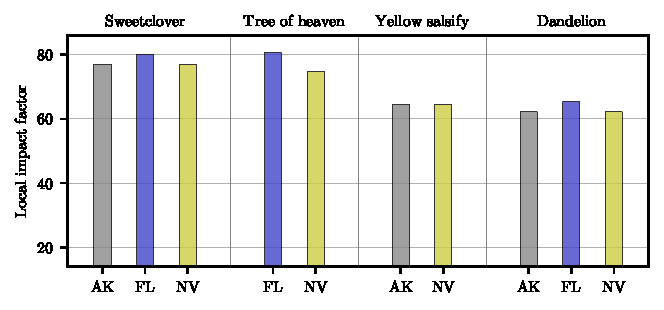
\includegraphics{IF_local-loc.pdf}
			\caption{Local impact factor}
			\label{fig:IFLocal}
		\end{figure}
		
	\subsection{Strengths and Weaknesses}

		some random text

\newpage	
\section*{We Share the Earth}
\addcontentsline{toc}{section}{We Share the Earth}


\newpage
\newrefcontext
\printbibliography

\end{document}
